\subsection{Plataforma \jason} \label{sec:aoppj}

A presente seção visa explicar a plataforma \jason baseada na arquitetura BDI.
Assim, na seção \ref{sec-jason-overview} uma visão geral é apresentada.
A engenharia da plataforma é discutida na seção \ref{sec-jason-architecture}.

\subsubsection{Visão Geral} \label{sec-jason-overview}

Para uma explicação mais didática será utilizado o
exemplo \emph{Room} que acompanha \emph{Jason}. Para isso será introduzido
o arquivo de projeto do exemplo e, a partir desse, os demais arquivos.
A Listagem~\ref{lst-roomMas2j} contém o arquivo de projeto.
Na linha 2, \emph{room} é o nome do projeto e, por isso, pode ser qualquer
identificador. A partir da linha 3 os valores antes dos dois-pontos (:)
são palavras reservadas que o \jason entende para diferentes propósitos e o valor
a seguir (depois dos dois-pontos) é o valor associado.
Assim, \emph{infrastructure}, na linha 3, pode assumir três valores
possíveis: (i) \emph{Centralised}, normalmente utilizada;
(ii) \emph{Jade}, utilizada quando se deseja integrar
com agentes não \jason (jade); (iii) \emph{Saci}, utilizada
quando deseja executar os agentes de maneira distribuída na rede.

\begin{center}
    \begin{minipage}{120mm}
	\begin{lstlisting}[frame=trbl, caption=Arquivo de projeto do \jason para o exemplo \emph{Room}, label=lst-roomMas2j]
// Isso eh um comentario
MAS room {
  infrastructure: Centralised
  environment: RoomEnv
  executionControl: jason.control.ExecutionControl
  agents: porter; claustrophobe; paranoid;
}
	\end{lstlisting}
    \end{minipage}
\end{center}

Continuando na Listagem~\ref{lst-roomMas2j}, a entrada \emph{environment}
configura a classe de ambiente que será utilizada. A próxima entrada,
normalmente não aparece, é a \emph{executionControl} utilizada para
mudar a forma com que os agentes são executados. O valor no exemplo é uma
classe que obriga o próximo ciclo de deliberação somente acontecer quando
todos os agentes terminaram o seu ciclo. O valor padrão é iniciar um novo
ciclo de deliberação após 500ms do ciclo de deliberação anterior ter sido
concluído, porém, algumas vezes isso
pode vir a apresentar problemas de sincronismo e, por isso, é interessante
mostrar que há uma opção para controlar a forma de execução dos ciclos
deliberativos. O usuário, inclusive, pode colocar sua própria classe como
configuração.

Todas as entradas apresentadas até agora mapeiam para código Java.
Os agentes são especificados na entrada \emph{agents}. Como pode-se
observar na Listagem~\ref{lst-roomMas2j}, cada referência a um agente deve
terminar com um ponto-e-vírgula (;). Há ainda como especializar cada um dos
agentes mudando opções. Na seção~\ref{sec-jason-architecture} e no
capítulo~\ref{ch:cdu} são mostrados exemplos dessas opções.

Os agentes são desenvolvidos em arquivos texto com extensão \emph{ASL}, porém
antes de entrar em discussão sobre os agentes será explicado o exemplo sendo
utilizado. No cenário desse exemplo tem-se uma porta na sala e duas pessoas, uma
claustrofóbica e outra paranoica. A pessoa claustrofóbica deseja que a
porta da sala esteja aberta, enquanto que a paranoica deseja que a porta
fique fechada.

Logo, há três agentes na linha 6 da Listagem~\ref{lst-roomMas2j}:
(i) \emph{porter} é o agente responsável pela porta e o único que conhece
como abri-lá ou fecha-lá;
(ii) \emph{claustrophobe} é o agente que deseja deixar a porta sempre aberta;
(iii) \emph{paranoid} é o agente que deseja deixar a porta sempre fechada.
A implementação desses agentes torna-se simples com o uso de eventos.

Esses eventos podem ser de adição (+) ou de remoção (-) de crenças, metas ou
consultas. Todas as estruturas são semelhantes a chamada de função. No
exemplo ``telefone(808080822)'', telefone pode ser uma crença ou uma ação de
ambiente que pode ser executada dependendo de onde a entrada se localiza.
Note que, se essa entrada for precedida pelo sinal de exclamação (!) ou de
interrogação (?) então o significado é alterado respectivamente para uma meta
ou uma consulta. Ainda há a possibilidade de preceder uma crença ou meta
com sinal de adição ou de subtração significando ou adicionar/remover uma
crença ou estar recebendo/removendo uma crença, meta ou consulta.

\lstset{linewidth=75mm}
\begin{wrapfigure}{l}{85mm}
	\begin{lstlisting}[frame=trbl, caption=Agentes em ASL, label=lst-agente]
// claustrophobe.asl
+locked(door) : true
  <- .send(porter,achieve,~locked(door)).

// paranoid.asl
+~locked(door)
  <- .send(porter,achieve,locked(door)).

// porter.asl
+!locked(door)[source(paranoid)]
  : ~locked(door)
  <- lock.

+!~locked(door)[source(claustrophobe)]
  : locked(door)
  <- unlock.
	\end{lstlisting}
\end{wrapfigure}
%
Na Listagem~\ref{lst-agente} tem-se a continuação do exemplo e, por
simplicidade, todos os fontes dos agentes encontram-se reunidos. O agente denominado
\emph{claustrophobe} será o primeiro a ser detalhado e corresponde as linhas 1 até 3
da Listagem~\ref{lst-agente}. A programação em \jason é
guiada por reatividade nas crenças e percepções do próprio agente, assim, é necessário
uma forma de estruturar as ações à serem decididas. Essa forma é o plano.
O plano pode ser ativado quando se deseja adicionar, consultar ou remover \footnote{Uma remoção pode ser o momento de conter uma falhar, porém isso não será abordado.}
 uma crença ou meta. O plano da linha 2 até 3 da
Listagem~\ref{lst-agente} será detalhado adiante.

Em um plano há sempre três divisões: gatilho do evento, contexto e corpo.
A primeira e única à ser explicita é o gatilho do evento, que deve ocorrer para
o plano ser disparado. No exemplo ele está limitado do carácter inicial até
o dois-pontos (:). A divisão de contexto é onde se coloca as ações, crenças
ou regras de inferência que tem que ser válidas para o corpo do plano ser
considerado válido. Dessa forma, é
importante tomar cuidado no que vai no contexto em razão dele sempre ser
executado previamente para definir quais planos devem ser descartados.
A segunda divisão vai até a seta (<-) e não é obrigatória.
A terceira divisão, também não é obrigatória, possui todas as ações a serem
executadas quando o plano tornar-se ativo. No exemplo o plano tem em seu corpo
uma ação interna do \jason denominada \emph{send} que envia determinado dado
(terceiro parâmetro) para o agente especificado (primeiro parâmetro) com
determinado formato (segundo parâmetro).

Cabe chamar atenção para uma coisa, as ações internas podem ser definidas pelo
usuário. Uma ação interna possui o seguinte formato ``tcp.send'', assim essa
ação está definida no pacote \emph{tcp} pela classe \emph{send} que
deve especializar a classe \emph{DefaultInternalAction} do \emph{Jason}.
Entretanto, uma ação interna definida pelo \jason não possui indicativo de
pacote que é o caso do ``.send'' presente no código dos agentes.

No exemplo da linha 3 na Listagem~\ref{lst-agente}, o agente
\emph{claustrophobe} está enviando uma mensagem para o agente denominado \emph{porter}
ter a meta (\emph{achieve} no segundo parâmetro) de não ($\sim$) ter a crença
da porta estar fechada. Analogamente, o agente denominado \emph{paranoid}, definido
na linha 5 à 7, envia como crença ter a porta fechada. Logo, o agente \emph{porter} pode ser entendido
em sua quase totalidade na Listagem~\ref{lst-agente}. Um entendimento completo
do exemplo vem com o aprendizado das anotações que são dados que podem
ser guardados juntos das crenças e essas anotações podem ter suas anotações também.
No agente \emph{porter} essas anotações são utilizadas somente
para dizer que determinado plano só é válido quando tiver como fonte 
(do inglês \emph{source}) um determinado agente. O presente exemplo possui
as anotações, pois assume a hipótese do mundo aberto. Vale observar que, essas
anotações podem ser removidas sem nenhum problema adicional, visto que, no
mundo proposto o agente \emph{porter} recebe a meta a ser alcançada de um dos
dois agentes existentes.

A execução dos agentes acontece de forma arbitrária e deve-se ter em conta
que o primeiro agente que irá enviar a mensagem para o agente \emph{porter} dependerá
de como o mundo inicia. Logo, se o mundo iniciar com a porta fechada o primeiro
a enviar a solicitação será o agente \emph{claustrophobe}. Já se o mundo for iniciado
com a porta aberta o primeiro a enviar solicitação será o agente \emph{paranoid}.
Além disso, conforme a simulação vai correndo, os dois agentes ficam alternando
mensagens com o agente \emph{porter} por causa do compartilhamento do mesmo
recurso (a porta).

\subsubsection{Infra-estrutura do \jason} \label{sec-jason-architecture}

A plataforma \jason tem uma base de software completamente extensível como
é possível observar mediante a Figura \ref{fig-jason-infra-1}.
Nessa figura, a infra-estrutura encontra-se representada como um barramento
na parte inferior. Ela pode ser configurada através da chave de configuração
\emph{infrastructure} no arquivo de projeto (ver Listagem~\ref{lst-roomMas2j}).

A infraestrutura define todas as classes padrões que o usuário irá utilizar,
por exemplo observe que o barramento liga-se a dois adaptadores: um do tipo
agente e um de ambiente. Esses adaptadores permitem a compatibilidade entre
implementações distintas de classes permitindo que as implementações não
padrão variem sem ter que alterar a estrutura do barramento.

\begin{figure}
               \begin{center}
               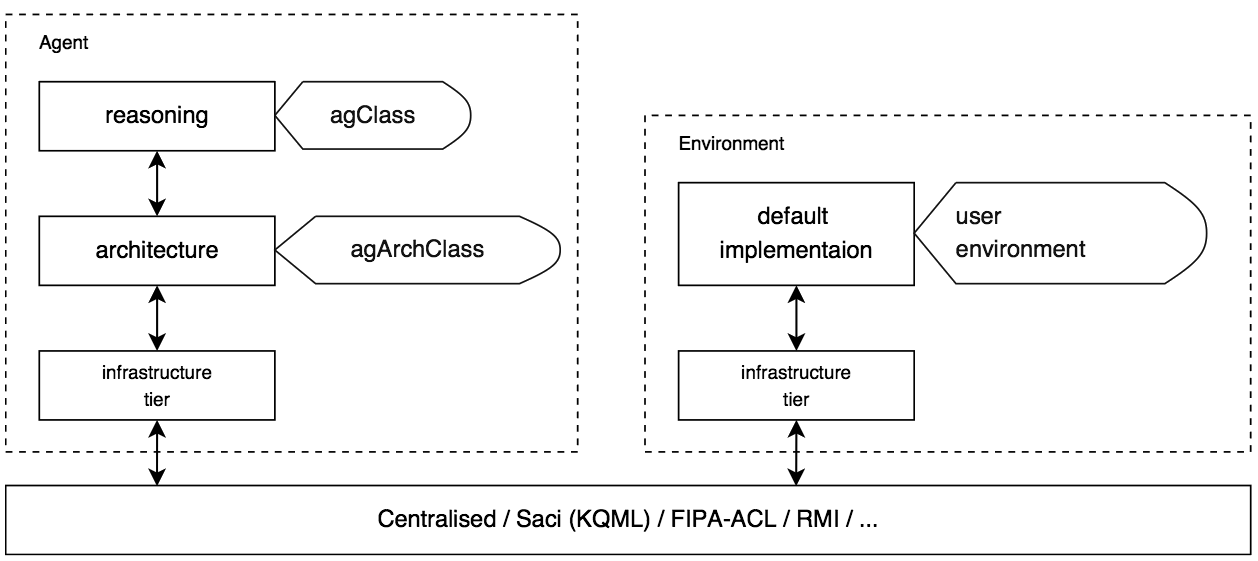
\includegraphics[width=140mm]{figuras/infra.png} 
                \end{center}
                \caption{Modelo da infra-estrutura do \emph{Jason}.}
                \label{fig-jason-infra-1}
\end{figure}

Assim, há a possibilidade de informar para uma determinada simulação que um
determinado agente utilizará uma arquitetura e/ou um raciocinador diferente
dos demais agentes. Para se fazer isso no momento que se declara os agentes
no projeto informa-se as chaves que encontram-se dentro das caixas com
cantos arqueados na Figura~\ref{fig-jason-infra-1}. O exemplo
``fb agArchClass KosMos.FireBrigadeArch agClass KosMos.Agent \#1;'' define
o agente \emph{fb} com a arquitetura usando a classe \emph{FireBrigadeArch}
do pacote \emph{KosMos} (pode ser qualquer nome desejado) e utilizando como
raciocinador a classe \emph{Agent} do mesmo pacote. Note que, essas classes
não existem no \jason e devem ser providas pelo usuário de alguma forma.

Como já explicado, a entrada \emph{environment} no arquivo de projeto
configura a classe de ambiente que será utilizada. Assim, somente um
é permitido por simulação. Um dos motivos comuns de se implementar um
ambiente é implementar as ações que o agente poderá realizar no mesmo. Aliás,
também, é possível alterar como os agentes ``visualizam'' o meio para, por
exemplo, inserir percepções incorretas em alguns momentos.
%
%% -> Esse paragrafo comentado parece que caiu de paraquedas...
%Um agente pode ser implementado deixando as ações tanto em uma
%especialização da infraestrutura quanto direto no ambiente. Por ser o
%ambiente, o responsável pelas percepções então seria nele que a implementação
%de falhas em sensores ocorreria. Essas falhas podem ser implementadas através
%da remoção ou alteração das percepções. O agente, nesse ambiente, deveria ser
%capaz de aplicar regras para verificar essas falhas e assumir que há erros em
%seus dados.

